\documentclass{article}
\usepackage[utf8]{inputenc}
\usepackage{titling}
\usepackage{enumitem}
\usepackage{graphicx}
\usepackage{xcolor}
\usepackage[colorlinks=true,linkcolor=darkgray, urlcolor =gray]{hyperref}
\usepackage[spanish]{babel}
\DeclareUnicodeCharacter{301}{~}
\usepackage{url}


\title{Práctica 5. GENIE como herramienta de ayuda al diagnóstico}
\author{Cristina Díaz García}
\date{Abril 2019}

\renewcommand\maketitlehooka{\null\mbox{}\vfill}
\renewcommand\maketitlehookd{\vfill\null}


\begin{document}

\addcontentsline{toc}{section}{Índice general}

\begin{titlingpage}
\maketitle
\end{titlingpage}

\newpage

\tableofcontents

\newpage

\section{Enunciado}

\textbf{\underline{Tarea:}} Resuelve los ejercicios propuestos. 

\textbf{\underline{Entrega:}} Documento pdf con la solución (capturas de pantalla y textos descriptivos)

\section{\textbf{Ejercicio 1}}

En el ejemplo del tutorial, diagnostica ahora el caso de un paciente que tiene un resultado de la prueba anormal y que fuma. Captura la pantalla de las enfermedades, y explica cual es ahora la enfermedad más probable para este paciente.

\subsection{Solución}

\begin{center}
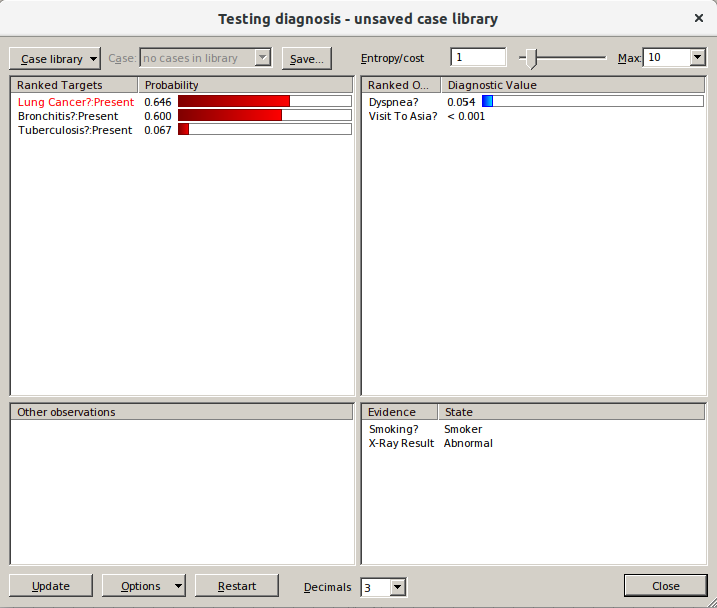
\includegraphics[scale=0.5]{asia.png}
\end{center}

Lo más probable es que el paciente tenga cáncer de pulmón, aunque la probabilidad de que solo sea bronquitis no es mucho menor (casi 65\% de cáncer contra 60\% de bronquitis.)

\section{\textbf{Ejercicio 2}}

Carga la red Hepar-II que encontrarás en la carpeta Examples (dentro del directorio en el que esté GeNIe) y responde a las siguientes preguntas:

\begin{enumerate}[label=\alph*)]
\item ¿Qué nodos se han seleccionado como nodos objetivo? ¿Y cómo nodos auxiliares? ¿A qué nodos se les ha asignado el subtipo “Ranked”? Y de estos nodos etiquetados como “Ranked” ¿qué estados se han seleccionado como objetivos? (Nota: utiliza la vista \textit{"Spreadsheet"})
\item Utiliza la ventana de diagnóstico para estudiar las siguientes situaciones: supongamos un paciente que tiene alto el colesterol total (a999\_350) y los triglicéridos totales (a17\_4). ¿Cuál es la enfermedad que tiene mayor probabilidad en el caso de que dicho paciente sea hombre, y con qué probabilidad la padece? ¿Y en el caso en que sea mujer?. ¿Qué prueba conviene realizarle a cada uno de ellos a continuación si se quiere demostrar que tiene dicha enfermedad? ¿Cuánto cambian las probabilidades si se realiza dicha prueba y se obtiene que el resultado es positivo?
\end{enumerate}

\subsection{Solución}

\begin{enumerate}[label=\alph*)]
\item ¿Qué nodos se han seleccionado como nodos objetivo? ¿Y cómo nodos auxiliares? ¿A qué nodos se les ha asignado el subtipo “Ranked”? Y de estos nodos etiquetados como “Ranked” ¿qué estados se han seleccionado como objetivos? (Nota: utiliza la vista \textit{"Spreadsheet"})

\begin{flushleft}
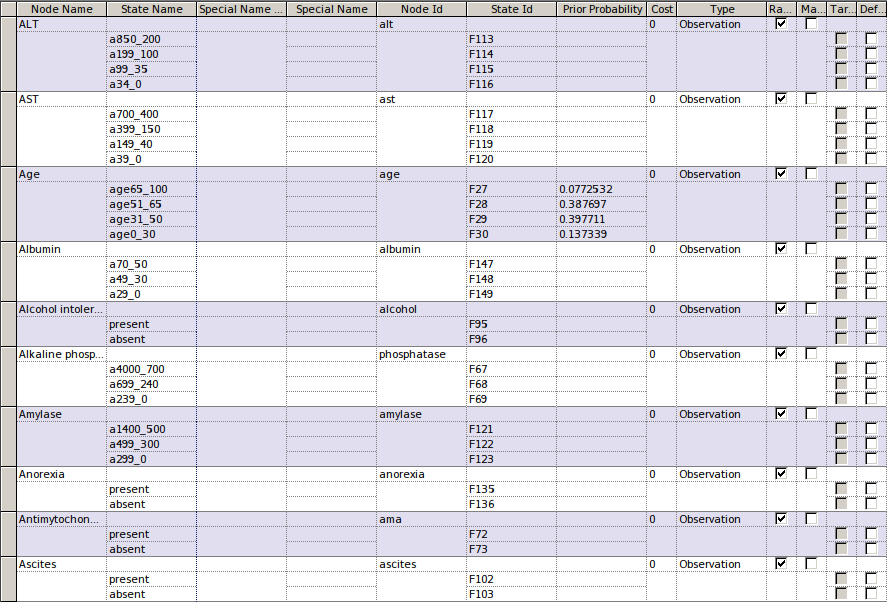
\includegraphics[scale=0.4]{hepa1.png}
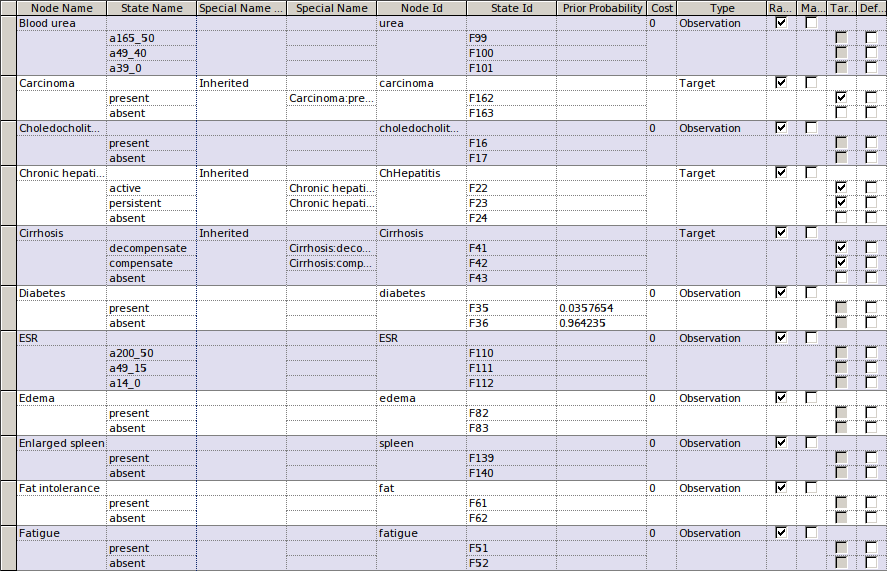
\includegraphics[scale=0.4]{hepa2.png}
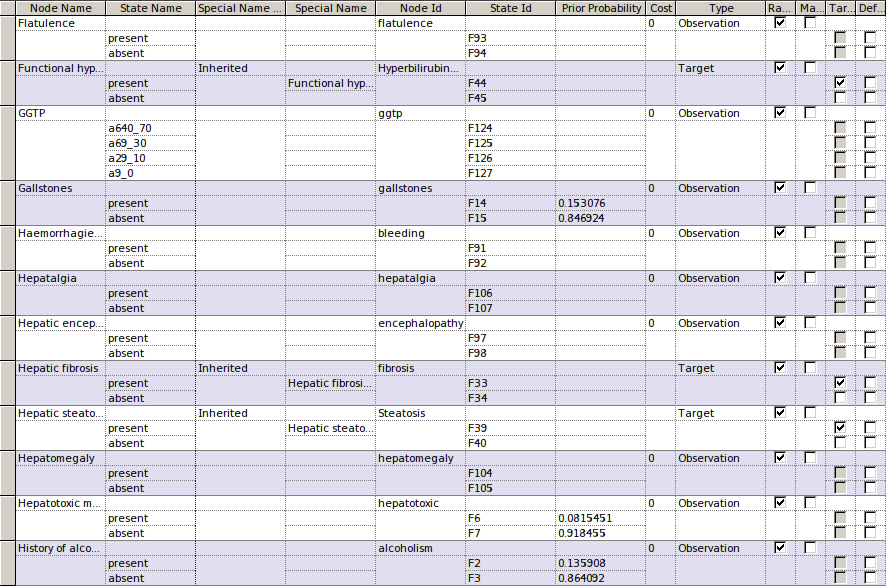
\includegraphics[scale=0.4]{hepa3.png}
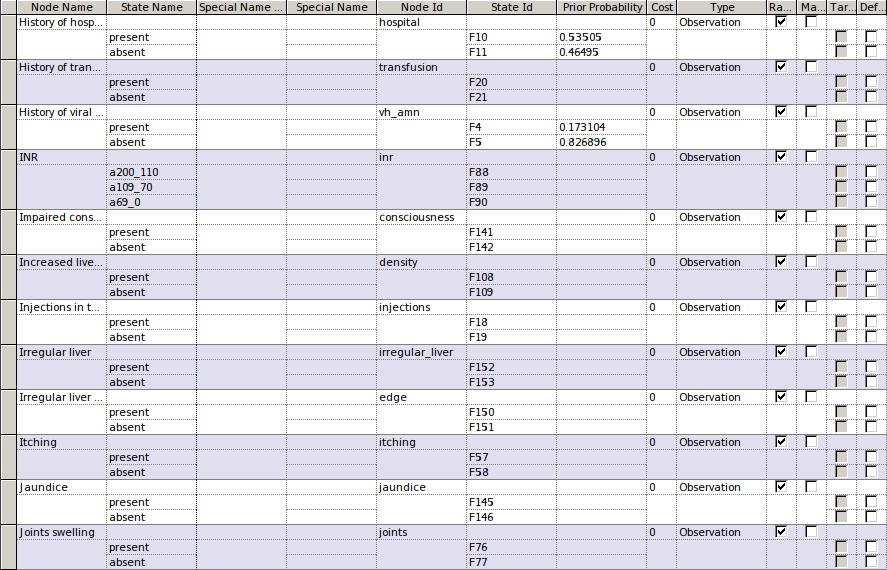
\includegraphics[scale=0.4]{hepa4.png}
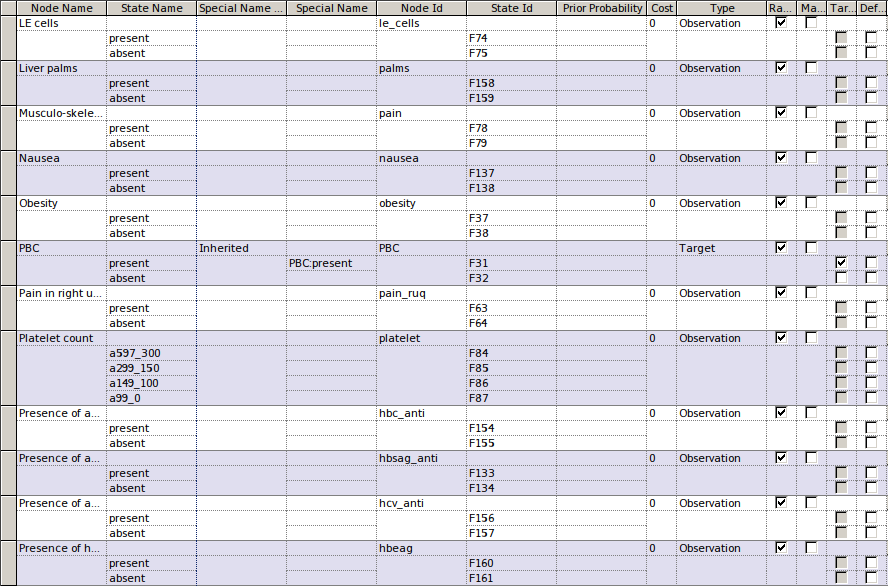
\includegraphics[scale=0.4]{hepa5.png}
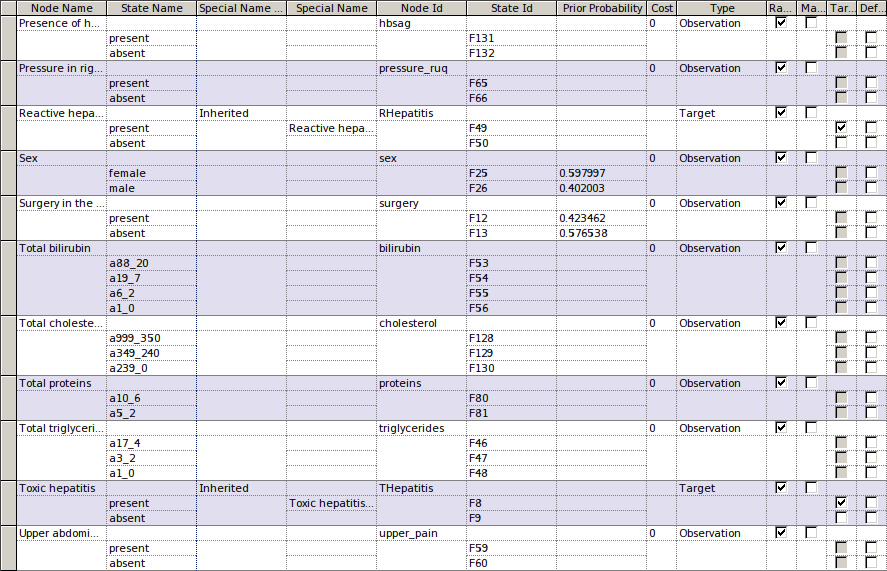
\includegraphics[scale=0.4]{hepa6.png}
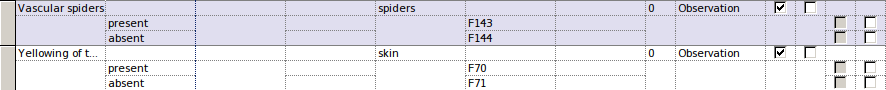
\includegraphics[scale=0.4]{hepa7.png}
\end{flushleft}

Como objetivo están seleccionados las enfermedades como tal: carcinoma, hepatitis crónica, cirrosis, esteatosis hepatica, fibrosis hepatica, hepatitis tóxica, hepatitis reactiva, PBC y hiperbilirrubinemia funcional. El resto son nodos auxiliares. Todos están seleccionados como \textit{ranked}, pero solo las opciones que no eran “ausente” de los nodos objetivos están seleccionadas como objetivo.

\item Utiliza la ventana de diagnóstico para estudiar las siguientes situaciones: supongamos un paciente que tiene alto el colesterol total (a999\_350) y los triglicéridos totales (a17\_4). ¿Cuál es la enfermedad que tiene mayor probabilidad en el caso de que dicho paciente sea hombre, y con qué probabilidad la padece? ¿Y en el caso en que sea mujer?. ¿Qué prueba conviene realizarle a cada uno de ellos a continuación si se quiere demostrar que tiene dicha enfermedad? ¿Cuánto cambian las probabilidades si se realiza dicha prueba y se obtiene que el resultado es positivo?

\newpage

Para el caso del hombre, la salida es la siguiente:

\begin{flushleft}
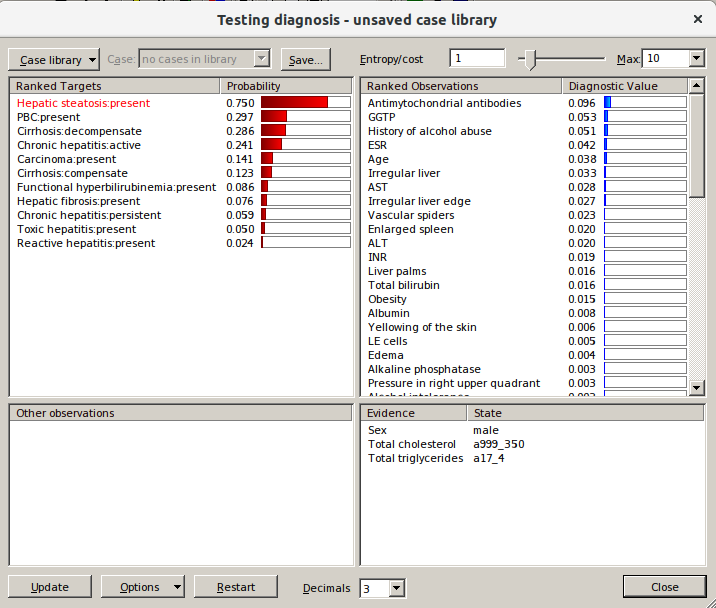
\includegraphics[scale=0.4]{hepaSOL.png}
\end{flushleft}

Para confirmar o descartar la esteatosis hepatica, lo siguiente que deberíamos haccer es realizarle una prueba de anticuerpos antimitocondriales. Tras la prueba, los resultados son:

\begin{flushleft}
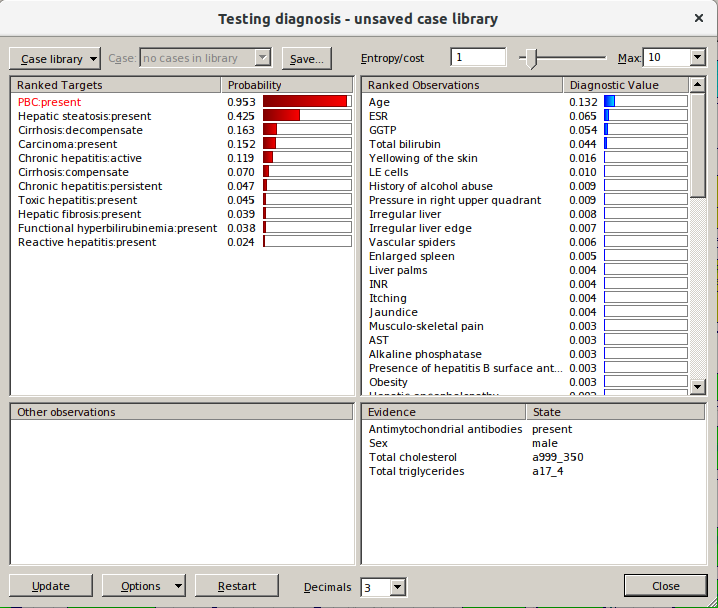
\includegraphics[scale=0.4]{hepasol.png}
\end{flushleft}

Por lo que el diagnóstico cambia a PBC.

En el caso de la mujer, la salida es la siguiente:
\begin{flushleft}
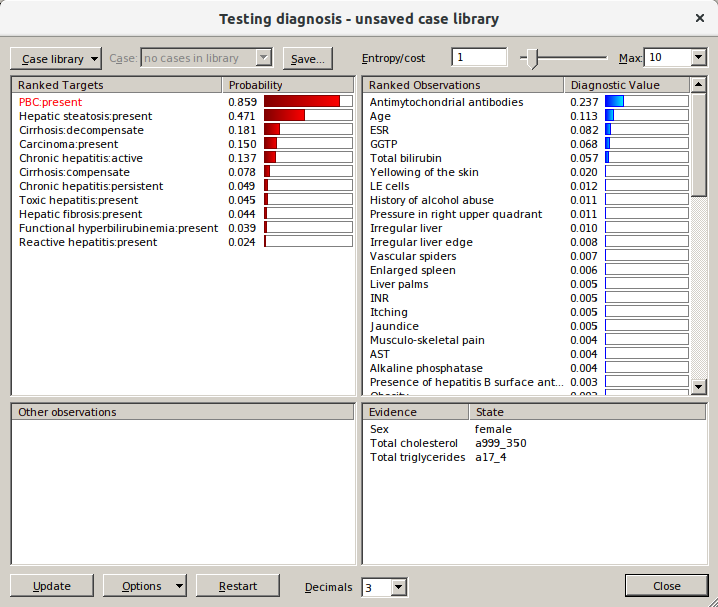
\includegraphics[scale=0.4]{hepaSOL2.png}
\end{flushleft}

Para confirmar o descartar el PBC, lo siguiente que deberíamos haccer es realizarle una prueba de anticuerpos antimitocondriales. Tras la prueba, los resultados son:

\begin{flushleft}
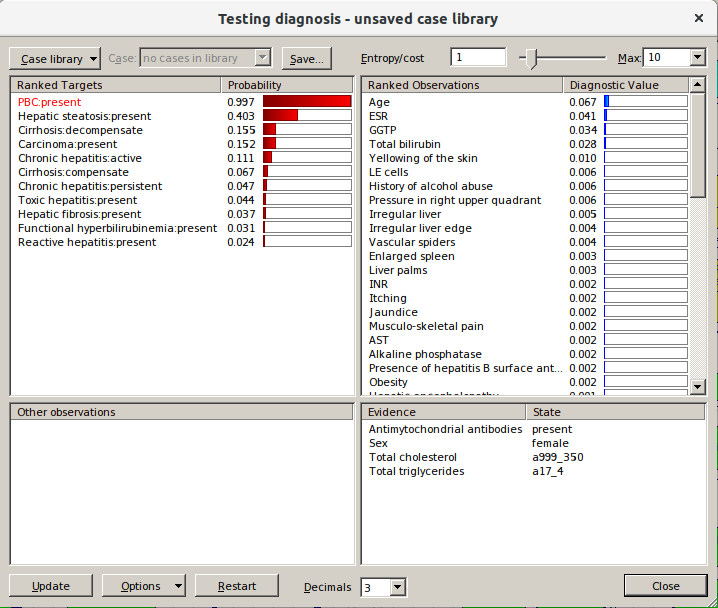
\includegraphics[scale=0.4]{hepasol2.png}
\end{flushleft}

Con lo que parece que se confirma el PBC.
\end{enumerate}

\section{\textbf{Ejercicio Opcional}}

GeNIe permite guardar casos que han sido diagnosticados con una red, y estos casos se pueden utilizar luego (por ejemplo, para hacer aprendizaje y mejorar los parámetros de la red). Para ello se utiliza la opción Case Manager, que vas a explorar con ayuda de este tutorial.
Para la entrega, abre de nuevo la red Hepar\_II, y resuelve lo siguiente:
\begin{enumerate}[label=\alph*)]
\item Vamos a ir diagnosticando algunos pacientes, y mientras que introducimos sus datos, vamos a ir guardando sus casos:\\
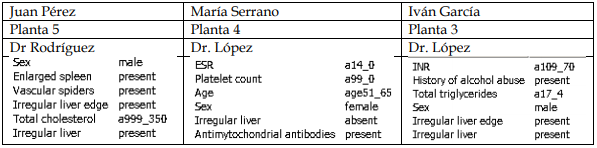
\includegraphics[scale=0.5]{tablaOpcional.png}
\\Para cada uno de ellos, indica qué enfermedad es más probable que padezcan, y con qué probabilidad.
\item Crea un nuevo caso (Juana Pérez), cargando el caso Iván García y modificando el sexo a mujer. ¿Cómo cambia el diagnóstico?
Si guardas la red con otro nombre (por ejemplo, Hepar II-cases), podrás comprobar que cuando la abres, si pinchas en la opción Case Manager, los casos se han guardado junto con la red.
\end{enumerate}

\subsection{Solución}

\begin{enumerate}[label=\alph*)]
\item Vamos a ir diagnosticando algunos pacientes, y mientras que introducimos sus datos, vamos a ir guardando sus casos:\\
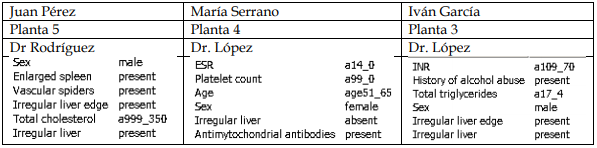
\includegraphics[scale=0.5]{tablaOpcional.png}
\\Para cada uno de ellos, indica qué enfermedad es más probable que padezcan, y con qué probabilidad.

\textbf{Juan Pérez}
\begin{flushleft}
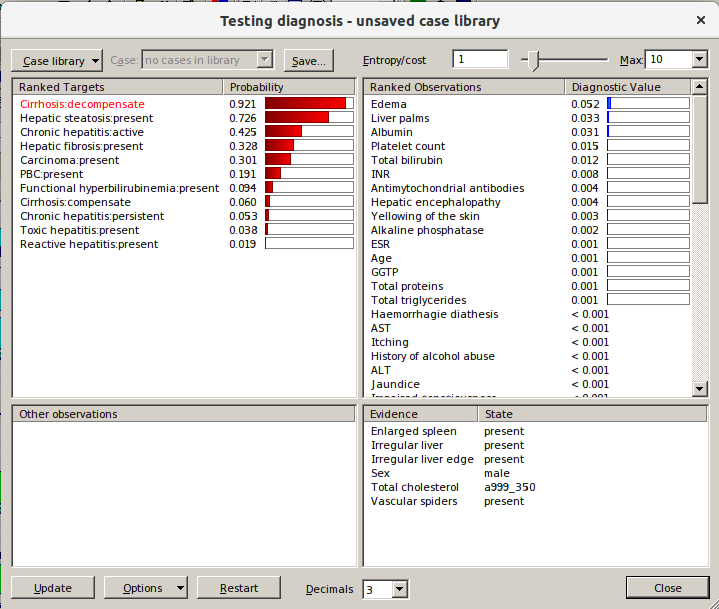
\includegraphics[scale=0.4]{Juan.png}
\end{flushleft}

Lo más probable es que Juan padezca cirrosis, con un 92.1\%.

\newpage

\textbf{María Serrano}
\begin{flushleft}
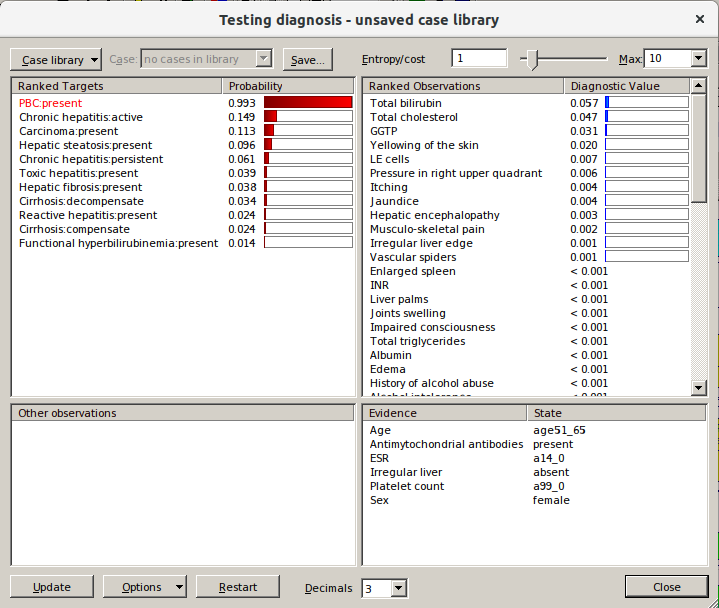
\includegraphics[scale=0.4]{Maria.png}
\end{flushleft}

Lo más probable es que María padezca PBC, con un 99.3\%.\\

\newpage

\textbf{Ivan García}
\begin{flushleft}
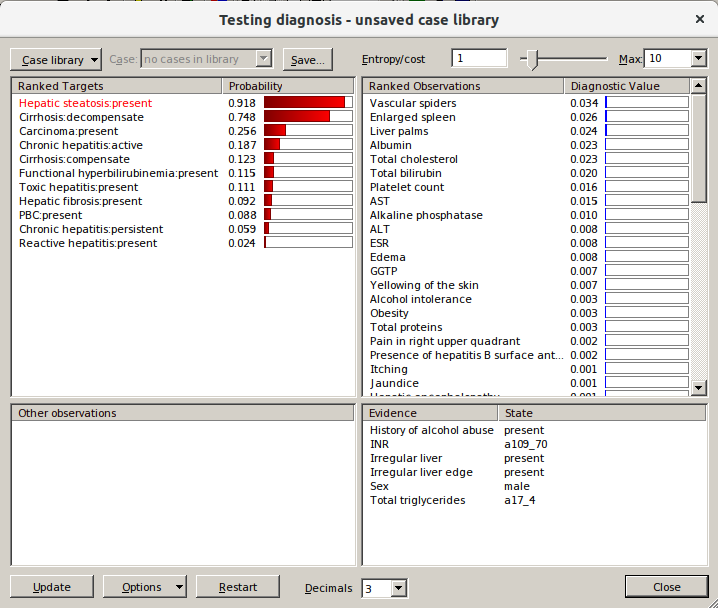
\includegraphics[scale=0.4]{ivan.png}
\end{flushleft}

Lo más probable es que Iván padezca esteatosis hepatica, con un 91.8\%.

\item Crea un nuevo caso (Juana Pérez), cargando el caso Iván García y modificando el sexo a mujer. ¿Cómo cambia el diagnóstico?\\
\newpage
\textbf{Juana Pérez}
\begin{flushleft}
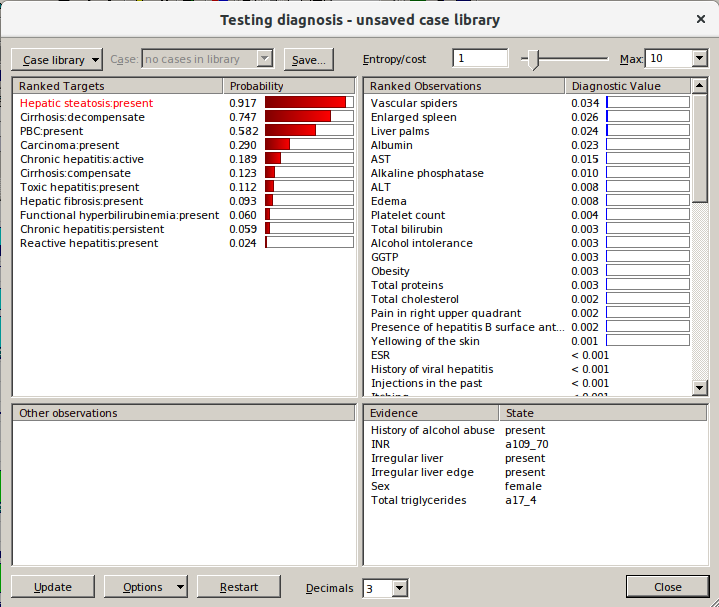
\includegraphics[scale=0.4]{Juana.png}
\end{flushleft}

El diagnóstico ahora es esteatosis hepatica, con un 91.7\%.

\end{enumerate}

\begin{thebibliography}{9}
\bibitem{Bayes} Información oficial de GeNIe, \url{https://www.bayesfusion.com}.
\end{thebibliography}

\end{document}